\documentclass{article}%
\usepackage[T1]{fontenc}%
\usepackage[utf8]{inputenc}%
\usepackage{lmodern}%
\usepackage{textcomp}%
\usepackage{lastpage}%
\usepackage{longtable}%
\usepackage{graphicx}%
\usepackage{fancyhdr}%
%
\fancypagestyle{header}{%
\renewcommand{\headrulewidth}{0pt}%
\renewcommand{\footrulewidth}{0pt}%
\fancyhead{%
}%
\fancyfoot{%
}%
\fancyhead[R]{%
Daffy Ducks%
\linebreak%
DSC 207: Mini{-}Project%
\linebreak%
Week 6 \& 7%
}%
\fancyfoot[C]{%
Page \thepage\ of \pageref{LastPage}%
}%
}%
%
\begin{document}%
\normalsize%
\pagestyle{header}%
\section{Mini{-}Project}%
\label{sec:Mini{-}Project}%
\textit{Goal: To explore the 2016.csv dataset and present findings using data analysis and visualization techniques.    In this mini{-}project, we will work with the dataset supplied and go through the data science process using the tools     and techniques learned from Weeks 1 {-} 5.The aim is to potentially use these tools together to achieve the objective of data exploration.}%
\subsection{High Level View {[}2 pts{]}}%
\label{subsec:HighLevelView2pts}%
\textit{Describe the dataset in words (50 words). Look at the data samples and describe what they represent and how they could be useful in a variety of data science tasks.}%
\begin{enumerate}%
\item%
The 2016.csv contains 13 fields, and 157 records.The dataset gives us 157 unique countries, that are split across 10 different regions. We are given some metrics for each country like  happiness score, freedom, government corruption, family,and generosity. This data set could be useful for looking at how government corruption or freedom varies by region and country. It could also be useful for determining which of the metrics given is most influential on happiness score.%
\end{enumerate}

%
\section{Data Exploration}%
\label{sec:DataExploration}%
\textit{In this step, you should explore what is present in the data and how the data is organized.    You are expected to answer the following questions using the pandas library and markdown cells to describe your actions:}%
\subsection{Preliminary Exploration}%
\label{subsec:PreliminaryExploration}%
\begin{enumerate}%
\item%
\textit{Are there quality issues in the dataset (noisy, missing data, etc.)?}%
\begin{itemize}%
\item%
Checking for inital quality issues int the dataset with df.info() where df is a pandas DataFrame object of our 2016.csv. Printing df.info gives us the following information:%
\begin{longtable}{l l l}%
\hline%
column name&total non{-}null values&data type\\%
\hline%
\endhead%
\hline%
country&157&object\\%
region&157&object\\%
happiness\_score&157&float64\\%
gdp\_per\_capita&157&float64\\%
family&157&float64\\%
life\_expectancy&157&float64\\%
freedom&157&float64\\%
government\_corruption&157&float64\\%
generosity&157&float64\\%
dystopia\_residual&157&float64\\%
\hline%
\multicolumn{3}{l}{Table 1 : Initial quality check of the 2016.csv dataset}\\%
\endlastfoot%
\end{longtable}%
\end{itemize}%
\item%
\textit{What will you need to do to clean and/or transform the raw data for analysis?}%
\begin{itemize}%
\item%
Checking for null values (df.isnull().sum())%
\item%
Dropping countries with a value 0 for an observation%
\item%
The happiness\_rank is an integer value that corresponds to the happiness\_score, such that the max happiness is given a happiness\_rank of 1, the min happiness is given a happiness\_rank of n where n is the total number of records.Therefore, we need to reset the happiness rank to account for these dropped countries with an observation of 0.%
\end{itemize}%
\item%
\textit{What are trends in the dataset using descriptive statistics (mean, median etc) and distribution of numerical data (eg. histograms)?}%
\begin{itemize}%
\item%
In order to idenitify the global and statical trends in the data we can isolate the numerical columns categorical columns. By sepearting the numerical variables into a pandas dataframe we can                 following descriptive statistics for each numerical variable: mean, median, and standard deviation.                 We can compare mean and median to determine if the data is skewed.%
\item%
By using histograms to visualize numerical data, we can see the distribution of the data. This will help us understand the data better and identify any skewness in these numerical variables.%
\end{itemize}%
\end{enumerate}

%
\subsection{Preliminary Exploration Tasks}%
\label{subsec:PreliminaryExplorationTasks}%
\textit{You are expected to show a minimum of 2 preliminary exploration tasks that you performed with justification. Typically, preliminary exploration helps us in identifying specific objectives for data analysis tasks.}%
\begin{itemize}%
\item%
Check for skewness in the data using histograms and descriptive statistics%
\begin{enumerate}%
\item%
In a distribution that is skewed right, the mean is greater than the median. While in a distribution that is skewed left, the mean is less than the median. For distrobutions                 that appear symmetric, the mean and median are roughly equal. By comparing the mean and median of the numerical variables in the 2016.csv dataset we can determine if a particular variable may contain outliers.%
\begin{longtable}{l l l}%
\hline%
column name&mean&median\\%
\hline%
\endhead%
\hline%
happiness\_score&5.382185&5.314\\%
gdp\_per\_capita&0.953880&0.982\\%
family&0.793621&0.810\\%
life\_expectancy&0.557619&0.606\\%
freedom&0.370994&0.397\\%
government\_corruption&0.137624&0.088\\%
generosity&0.242635&0.222\\%
dystopia\_residual&2.325807&2.290\\%
\hline%
\multicolumn{3}{l}{Table 2 : Mean and modes for numerical variables in the 2016.csv dataset}\\%
\endlastfoot%
\end{longtable}%
\item%
Histograms%


\begin{figure}[h!]%
\centering%
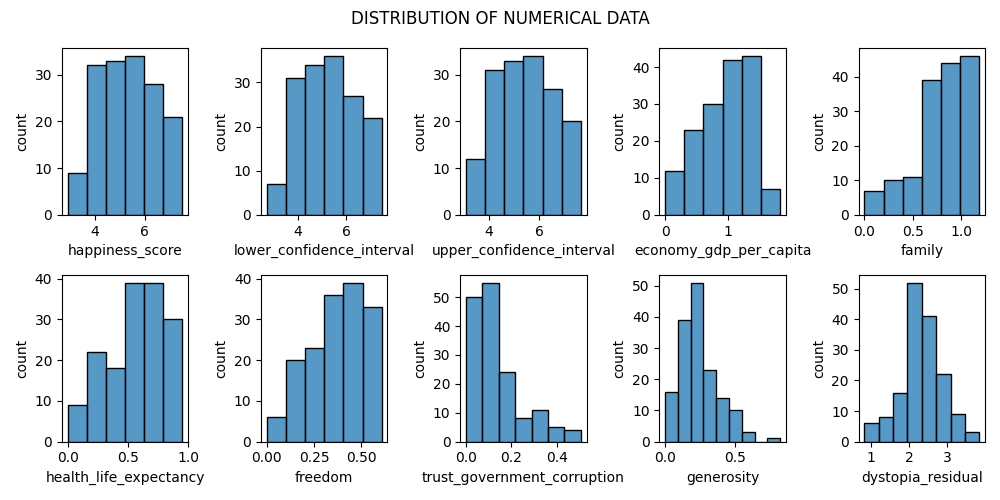
\includegraphics[width=300px]{/plots/dis_of_num_data.png}%
\caption{Figure 1 : Histograms of numerical data in the 2016.csv dataset}%
\end{figure}

%
\end{enumerate}%
\item%
Check for null values or missing data in the dataset%
\end{itemize}

%
\end{document}